\subsection{A* Search with heuristic}
\noindent A* algorithm is one of the popular technique used in path finding and graph traversals. This algorithm completely relies on heuristics for computing the future cost of a problem. This algorithm is equivalent to the uniform cost search with modified edge cost. This heuristics is chosen according to the case where the algorithm is implemented, thus emphasizing the importance of domain knowledge. This algorithm is consistent if the modified cost is greater than zero.

\begin{figure}[H]
	\centering
	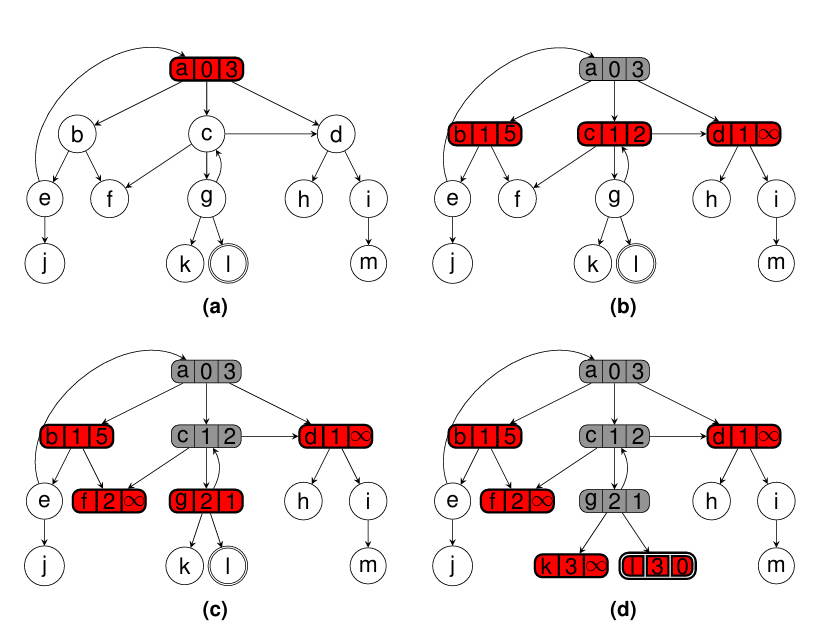
\includegraphics[width=0.8\textwidth]{./imgs/astar.png}
	\caption{A* Algorithm}
\end{figure}

\subsubsection{Pseudocode}
\begin{algorithm}[H]
	\caption{A* Search with heuristic (\textit{state, maxdepth, maxtimeout})}
	\label{alg:ucs}
	\begin{algorithmic}[1]
	\State priority queue $\gets$ starting position of Sokoban
	\State cost $\gets$ cost of moves
	\State Fix the Heuristics 
	\While {queue is not empty}
		\State Remove the highest priority element of queue
		\If {Ares crates on target}
			\State break
		\Else
			\If {Is deadlock or depth $\geq$ maxdepth or time $\geq$ maxtimeout}
				\State pick next solution
			\Else
				\State Get valid moves for Sokoban
				\ForAll {move}
					\State cost $\gets$ cost of move with heuristics
					\State Add cost to current move
					\State Update queue with new cost and new state
					\State Find Heuristics of new state
				\EndFor
			\EndIf
		\EndIf
	\EndWhile
	\State \Return moves
	\end{algorithmic}
\end{algorithm}

\subsubsection{Implementation}

\subsubsection{Time and Space Complexity}